\section{Linear parameter estimation} 
\label{LinParamEst}

%As can be seen in \eqref{multistate model_smallsignal}, the small signal model of such a multi-state/ multi-input system consists of two Jacobian matrices, one for the states and one for the inputs to the system. It should be emphasized however that these matrices have to be evaluated at the operating points, at $(\bar{x}, \bar{u})$. It is a reasonable statement since the inputs to the model are the small signal values of OD and differential pressures, dp, from the pumps. Therefore the same excitation to the real test setup can be carried out by taking the operating values into account and by adding them to the small signal values. 

\begin{figure}[H]
\centering
\input{report/tikz/param_block_lin.tex} 
\caption{Parameter identification block diagram for the linear system. }
\label{fig:parame_block_lin}
\end{figure}

\subsection{Measurements on the test set up}
\label{LinParamEst_measurements}

From the system setup $8$ different relative pressures can be measured, following \figref{systemdiagram} notation the sensors are placed in: 
$n_2$ $n_4$ $n_5$ $n_7$ $n_{10}$ $n_{11}$ $n_{15}$ $n_{16}$.

The measurements obtained from the pressure sensors placed in these nodes, are relative to the atmospheric pressure. Thus, in order to compare the measurements
from the system setup and the data obtained from the simulation in Matlab, an atmospheric pressure node, $n_1$, is set as reference point.

Therefore, the relationship between pressures, where DpCXX describes the pressure difference for the XX component, can be defined as:

\text{\underline{Node 2}} 
\vspace{4mm}
\begin{equation}
     y_1 = DpC2 
\end{equation}

\text{\underline{Node 7}}
\vspace{4mm}
\begin{equation}
   y_2 = DpC16 
\end{equation}

\text{\underline{Node 4}}
\vspace{4mm}
\begin {equation}
    y_3 = DpC18 + DpC19 + DpC23 + DpC24 
\end{equation}

\text{\underline{Node 5}}
\vspace{4mm}
\begin {equation}
    y_4 = DpC25 + DpC26 + DpC30 + DpC31 
\end{equation}

\text{\underline{Node 10}}
\vspace{4mm}
\begin {equation}
     y_5 = DpC20 + DpC21  
\end{equation}

\text{\underline{Node 11}}
\vspace{4mm}
\begin {equation}
     y_6 = DpC24
\end{equation}


\text{\underline{Node 15}}
\vspace{4mm}
\begin {equation}
     y_7 = DpC28 + DpC20 
\end{equation}

\text{\underline{Node 15}}
\vspace{4mm}
\begin {equation}
     y_8 = DpC31 
\end{equation}

As the parameter estimation is based on a linearized model an operating point for the system is chosen. This point is based on the tank level being approximately half way full which allows for an equal amount of deviation in both directions. Based on the chosen operating point, data is gather from the system while small steps are individually applied to the two main pumps and the opening degree of the pma valves. In order to use the data for parameter estimation the operating point is subtracted, leaving only small signal values.  

The operating point of the pma valves is chosen to $70^{\circ}$ and the small signal values for the estimation can be seen in \figref{fig:est_OD_data}.

\begin{figure}[H]
\centering
% This file was created by matlab2tikz.
%
%The latest updates can be retrieved from
%  http://www.mathworks.com/matlabcentral/fileexchange/22022-matlab2tikz-matlab2tikz
%where you can also make suggestions and rate matlab2tikz.
%
\definecolor{mycolor1}{rgb}{0.00000,0.44700,0.74100}%
\definecolor{mycolor2}{rgb}{0.85000,0.32500,0.09800}%
\definecolor{mycolor3}{rgb}{0.92900,0.69400,0.12500}%
\definecolor{mycolor4}{rgb}{0.49400,0.18400,0.55600}%
%
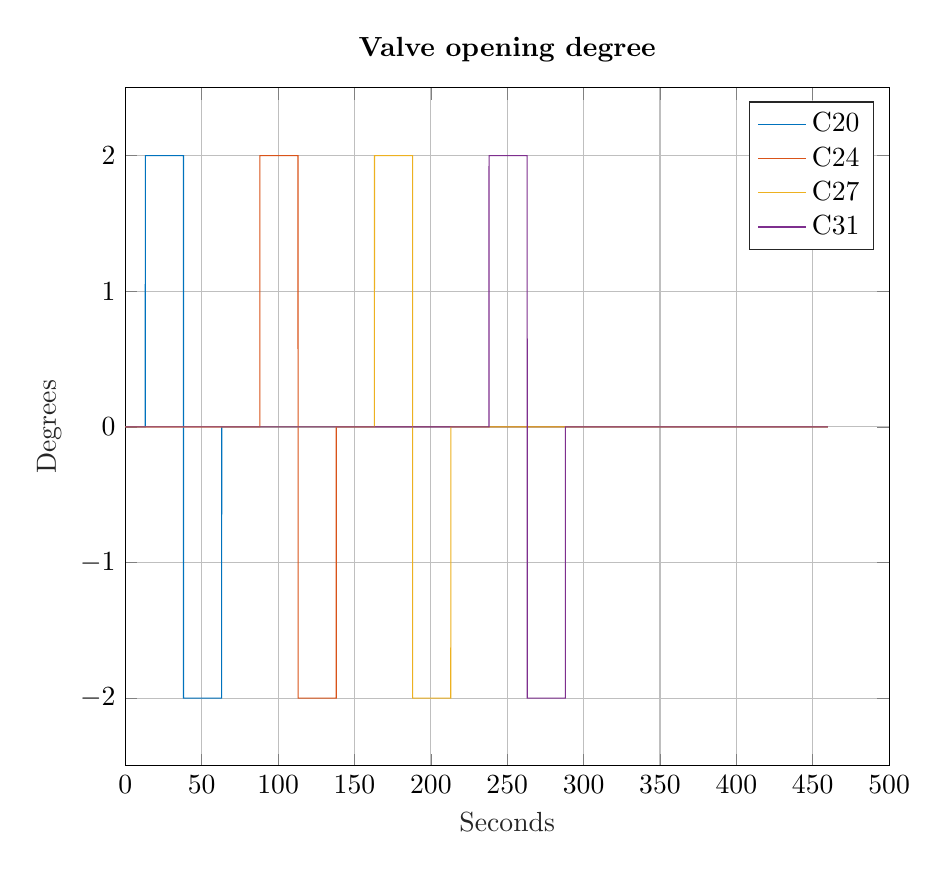
\begin{tikzpicture}

\begin{axis}[%
width=0.8\textwidth,
height=3.39in,
at={(0.758in,0.481in)},
scale only axis,
xmin=0,
xmax=500,
xlabel style={font=\color{white!15!black}},
xlabel={Seconds},
ymin=-2.5,
ymax=2.5,
ylabel style={font=\color{white!15!black}},
ylabel={Degrees},
axis background/.style={fill=white},
title style={font=\bfseries},
title={Valve opening degree},
xmajorgrids,
ymajorgrids,
legend style={legend cell align=left, align=left, draw=white!15!black}
]
\addplot [color=mycolor1]
  table[row sep=crcr]{%
0	-1.13686837721616e-13\\
13.05	-1.13686837721616e-13\\
13.1	1.99999999999989\\
38.05	1.99999999999989\\
38.1	-2.00000000000006\\
63.05	-2.00000000000006\\
63.1	-1.13686837721616e-13\\
459.95	-1.13686837721616e-13\\
};
\addlegendentry{C20}

\addplot [color=mycolor2]
  table[row sep=crcr]{%
0	-1.13686837721616e-13\\
88.05	-1.13686837721616e-13\\
88.1	1.99999999999989\\
113.05	1.99999999999989\\
113.1	-2.00000000000006\\
138.05	-2.00000000000006\\
138.1	-1.13686837721616e-13\\
459.95	-1.13686837721616e-13\\
};
\addlegendentry{C24}

\addplot [color=mycolor3]
  table[row sep=crcr]{%
0	-1.13686837721616e-13\\
163.05	-1.13686837721616e-13\\
163.1	1.99999999999989\\
188.05	1.99999999999989\\
188.1	-2.00000000000006\\
213.05	-2.00000000000006\\
213.1	-1.13686837721616e-13\\
459.95	-1.13686837721616e-13\\
};
\addlegendentry{C27}

\addplot [color=mycolor4]
  table[row sep=crcr]{%
0	-1.13686837721616e-13\\
238.05	-1.13686837721616e-13\\
238.1	1.99999999999989\\
263.05	1.99999999999989\\
263.1	-2.00000000000006\\
288.05	-2.00000000000006\\
288.1	-1.13686837721616e-13\\
459.95	-1.13686837721616e-13\\
};
\addlegendentry{C31}

\end{axis}
\end{tikzpicture}% 
\caption{Small signal values of the opening degrees of the pma valves. }
\label{fig:est_OD_data}
\end{figure}


Here the plots from Matlab could be inserted with the input signals, output pressures. The process of the data could be explained, where are the measurements...

\todo{Daniel, you have the things for this!}